\documentclass[../Main.tex]{subfiles} 
\begin{document}

\section{Geo location attempt }
As stated in the previous chapter, the foundation of all calculations in the regional word attempt is a list of a few hundred words that appear more likely in a specific region. 
Although this list and their probability distribution is based on scientific research it markes the weak spot of this attempt for number of reasons. For example people in a specific region use a typically word in their everyday language while speaking to their friends or family, but there is no proof that this people also use this words in their written language, even if it is only their private Twitter account. In addition, the list is way to short to cover only fraction of the words, people use on Twitter, so the end results mostly rely on the data that is generated in main loop of the algorithm.

We seem to have no other choice but to trust this generated values, so we had the idea of skipping the manually created word list and use an automatically created based on a corpus of Tweets with a geo location instead. \\
Before entering the main loop, we had to write another algorithm that learns the distribution on all seven regions for all the words in the corpus. This way we are generating a list of words that covers nearly all the words.
\begin{figure}
  \begin{center}
   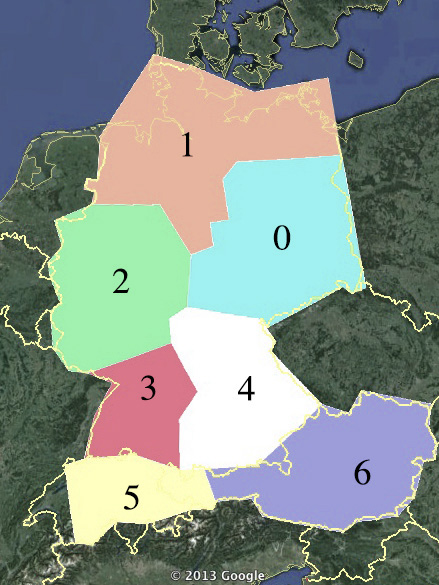
\includegraphics[width=0.5\columnwidth]{../img/polygone_satt.jpg}
    \caption{\label{geo_polymap} Map of the regions and their index represented as polygons}
  \end{center}
\end{figure}
In order to classify a tweet, that has a geo location, we had struggled to find a good way to represent the seven regions in a way, that we could easily check from which of them a Tweet was sent. After a few unsuccessful approaches, we decided to define polygons for the regions that are not overlapping each other, but also leave no gaps between them. For the value of the points we simply used their longitude and latitude coordinates, that can be represented as floats.  
We did not implement a point-in-polygon algorithm ourself, but used the version found here [SOURCE] instead. 
To find out from which region a tweet was sent, we iterate over all regions and return the first one, where the point-in-polygon function returns true.
In this first step, the Tweet-vector consists only of zeros and a one for the feature standing for the region it was sent from. 

Let's assume that the coordinates of some Tweet reveal, that its region is "Westdeutschland", represented by the index $3$.
Therefore the Tweet-vector is $(0,0,1,0,0,0,0)$. 
The next step consists of iterating over all token in the tweet and add the Tweet-vector to their word-vectors. To put it simply, we increase the counter for the specific feature of all occurring tokens by one. 
In the final step, we iterate over all word-vectors and use our \texttt{normalize()}-function to attain the probability distribution, how likely it is that the token is used in a specific region. Because of this normalization, the format of the outcome is comparable to the input list in the regional-word attempt and we can use the main part of the algorithm without having to adjust it.

\begin{figure}
\centering $\textrm{Example Tweet: } d = \textrm{'Hello Twitter!'} \textrm{ from the region 'Westdeutschland'.}$
 \begin{align*}
    \vec{t}_{hello} &= (1,3,2,5,2,1,0) \\
     \vec{t}_{twitter} &= (0,0,0,0,0,0,0) \\
      \vec{d} &= (0,0,1,0,0,0,0) \\
     \vec{t}_{hello}' &= \vec{t}_{hello} + \vec{d} =  (1,3,3,5,2,1,0) \\
    \vec{t}_{twitter} ' &= \vec{t}_{twitter} + \vec{d} = (0,0,1,0,0,0,0) \\
     \texttt{normalize(}\vec{t}'_{hello}\texttt{)} &= (0.04, 0.13, 0.13, 0.22, 0009, 0.04, 0) \\
     \texttt{normalize(}\vec{t}'_{twitter}\texttt{)} &= (0,0,1,0,0,0,0)
  \end{align*}
  \caption{Example for the creation of the initial word-vectors}
  \label{geo_example1}
\end{figure}

\subsection{Source of data}
The datasets used for the generation of the first word-vectors have been extracted from the Scheffler-corpus using the same classification function as in the main program. Although the corpus mostly consist of German Tweets (filtered with \emph{LangID}), about 20\% of the Tweets with geo-location have not been sent from one of the defined regions and therefore have been ignored. \\
We created balanced sets, where the amount of  Tweets are the same for all regions. Because the fewest number of Tweets (8787) came from region 6, 'Austria', we ended up with only 61509 Tweets for all regions. 

In order to create a gold-standard, we substracted 150 Tweets from each region, leaving us 60459 for the training. \\
Our assumption was, that datasets of different sizes lead to different results and we wondered, how it would effect the accuracy, if we would use the same data for the creation of the word-vectors and for the main-algorithm. Therefore we created three sets:
\begin{enumerate}
\item \emph{balanced-21k} with 3000 Tweets from each region.
\item \emph{balanced-39k} consisting of the remaining 39456 Tweets (no intersection with the \emph{balanced-21k} set)
\item \emph{balanced-61k} combining the both previous sets. 
\item \emph{unbalanced-175k} with all Tweets from the corpus that were sent from one of the defined regions. Not normalized.
\end{enumerate}
\subsection{Experiments}


\newpage

\subsubsection{Parameters}
\subsubsection{Expectations}
\subsubsection{Discussion}
\subsubsection{-> new Experiment}
\subsection{Conclusion}

\end{document}
